This section describes a number of test functions for
optimization. That functions are taken from the literature on both
local and global optimization.

%\subsection*{The De Jong's function}

%One of the simplest test functions for optimization is the De Jong's
%function, which is an unconstrained and unimodal function. The De
%Jong's function optimization problem in $d$ variables can be stated
%as:


%The De Jong's function has got a unique minimal argument
%$\boldsymbol\zeta^{*} = (0, \ldots, 0 )$, which gives a minimum value
%$f(\boldsymbol\zeta^{*}) = 0$. Figure \ref{DeJongFunction} is a plot of
%that function in $2$ variables.

%\begin{figure}[h!]
%\begin{center}
%\includegraphics[width=0.75\textwidth]{function_optimization/de_jong_function}
%\caption{The De Jong's Function in $2$ variables.}\label{DeJongFunction}
%\end{center}
%\end{figure}

%The gradient vector for the De Jong's function is given by and the Hessian matrix by

\subsection*{The Rosenbrock's function}

The Rosenbrock's function, also known as banana function, is an
unconstrained and unimodal function. The optimum is inside a long,
narrow, parabolic shaped flat valley. Convergence to that optimum is
difficult and hence this problem has been repeatedly used in assess
the performance of optimization algorithms. The Rosenbrock's
function optimization problem in $d$ variables can be stated as:

\begin{figure}[h!]
\begin{center}
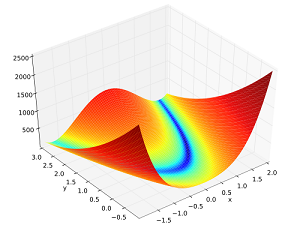
\includegraphics[width=0.75\textwidth]{function_optimization/rosenbrock_function.png}
\caption{The Rosenbrock's function in $2$
variables.}\label{RosenbrockFunction}
\end{center}
\end{figure}

The minimal argument of the Rosenbrock's function is found at
$(1, \ldots, 1)$. The minimum value of that
function is $= 0$. Figure \ref{RosenbrockFunction}
is a plot of the Rosenbrock's function in $2$ variables.

\subsection*{The Rastrigin's function}

The Rastrigin's function is based on the De Jong's function with the
addition of cosine modulation to produce many local minima. As a
result, this function is highly multimodal. However, the location of
the minima are regularly distributed. The Rastrigin's function
optimization problem in $d$ variables can be stated as:


\begin{figure}[h!]
\begin{center}
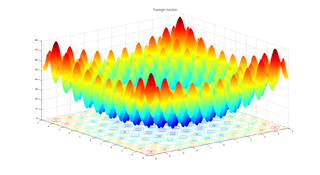
\includegraphics[width=0.75\textwidth]{function_optimization/rastrigin_function.png}
\caption{The Rastrigin's function in $2$
variables.}\label{RastriginFunction}
\end{center}
\end{figure}

The global minimum of the Rastrigin's Function is at $(0,\ldots,0)$. 
At this minimal argument the value of the function is
$0$. Figure \ref{RastriginFunction} is a plot of the
Rastrigin's function in $2$ variables.

The gradient vector for the Rastrigin's function is given by
\noindent and the Hessian matrix by


